\section{Linear Dimensionality Reduction}

\subsection{Principal Components Analysis  (10 points)}
\label{sec:pca}

Principal Components Analysis (PCA) is a popular method for linear dimensionality reduction. PCA attempts to find a lower dimensional subspace such that when you project the data onto the subspace as much of the information is preserved. Say we have data $X = [x_1^\top; \dots; x_n^\top] \in \RR^{n\times D}$ where  $x_i \in \RR^D$. We wish to find a $d$ ($ < D$) dimensional subspace $A = [a_1, \dots, a_d] \in \RR^{D\times d}$, such that $ a_i \in \RR^D$ and $A^\top A = I_d$, so as to maximize $\frac{1}{n} \sum_{i=1}^n \|A^\top x_i\|^2$.
\begin{enumerate}

\item  \textbf{(4 Points)}
Suppose we wish to find the first direction $a_1$ (such that $a_1^\top a_1 = 1$) to maximize $\frac{1}{n} \sum_i (a_1^\top X_i)^2$.
Show that $a_1$ is the first right singular vector of $X$.

\begin{soln}
Let $X = U\Sigma V^\top$ be the SVD of $X$. To find the first principal component, we need to find the direction in which the data varies the most, which means $a_1$ should be the solution of following optimization problem:
\begin{align*}
  \max_{a_1} \Var (Xa_1) &= (Xa_1)^T(Xa_1)/n = a_1^T \Sigma^T \Sigma a_1/n \\
  \text{s.t. } a_1^\top a_1 &= 1
\end{align*}
The solution of this problem will give the eigenvector associated with the largest eigenvalue of $\Sigma^T \Sigma$, which is the first right singular vector of $X$, to see that, we can exam that $X^\top X = V\Sigma^\top U^\top U\Sigma V^\top = V\Sigma^\top \Sigma V^\top$, and $\Sigma$ is a diagonal matrix with decreasing entries. Thus, the solution $a_1$ is the first right singular vector of $X$.
\end{soln}

\item  \textbf{(6 Points)}
Given $a_1, \dots, a_k$, let $A_k = [a_1, \dots, a_k]$ and 
$\tilde{x}_i = x_i - A_k A_k^\top x_i$. We wish to find $a_{k+1}$, to maximize
$\frac{1}{n} \sum_i (a_{k+1}^\top \tilde{x}_i)^2$. Show that $a_{k+1}$ is the
$(k+1)^{th}$ right singular vector of $X$.

\begin{soln}
  We can show it by induction. For $k=1$, we have already shown that $a_1$ is the first right singular vector of $X$. For $k$, $A_k$ is the first $k$ right singular vectors of $X$. We want to find $a_{k+1}$ to solve the following optimization problem:
  \begin{align*}
    \max \Var (\tilde{X}a_{k+1}) &= (\tilde{X}a_{k+1})^T(\tilde{X}a_{k+1})/n = a_{k+1}^T \tilde{\Sigma}^T \tilde{\Sigma} a_{k+1}/n \\
    \text{s.t. } a_{k+1}^\top a_{k+1} &= 1
  \end{align*}
  Where $\tilde{X} = [\tilde{x}_1^\top; \dots; \tilde{x}_n^\top] = X V_k V_k^\top$ and $\tilde{\Sigma}$ is $\Sigma$ with first $k$ diagonal entries are 0. Then the solution of this optimization problem is the $(k+1)^{th}$ right singular vector of $X$ since it associated with the largest entry of $\tilde{\Sigma}^T \tilde{\Sigma}$.
\end{soln}

\end{enumerate}


\subsection{Dimensionality reduction via optimization (22 points)}

We will now motivate the dimensionality reduction problem from a slightly different
perspective. The resulting algorithm has many similarities to PCA.
We will refer to method as DRO.

As before, you are given data $\{x_i\}_{i=1}^n$, where $x_i \in \RR^D$. Let $X=[x_1^\top; \dots
x_n^\top] \in \RR^{n\times D}$. We suspect that the data
actually lies approximately in  a $d$ dimensional affine subspace.
Here $d<D$ and $d<n$.
Our goal, as in PCA, is to use this dataset to find a $d$ dimensional representation $z$ for each $x\in\RR^D$.
(We will assume that the span of the data has dimension larger than
$d$, but our method should work whether $n>D$ or $n<D$.)


Let $z_i\in \RR^d$ be the lower dimensional representation for $x_i$ and
let $Z = [z_1^\top; \dots; z_n^\top] \in \RR^{n\times d}$.
We wish to find parameters $A \in \RR^{D\times d}$, $b\in\RR^D$ and the lower
dimensional representation $Z\in \RR^{n\times d}$ so as to minimize 
\begin{equation}
J(A,b,Z) = \frac{1}{n} \sum_{i=1}^n \|x_i - Az_i - b\|^2 = \| X - ZA^\top - \one b^\top\|_F^2.
\label{eqn:dimobj}
\end{equation}
Here, $\|A\|^2_F = \sum_{i,j} A_{ij}^2$ is the Frobenius norm of a matrix.


\begin{enumerate}
\item \textbf{(3 Points)}
Let $M\in\RR^{d\times d}$ be an arbitrary invertible matrix and $p\in\RR^{d}$ be an arbitrary vector.
Denote, $A_2 = A_1M^{-1}$, $b_2 = b_1- A_1M^{-1}p$ and $Z_2 = Z_1 M^\top +
\one p^\top$.
Show that both
$(A_1, b_1, Z_1)$ and $(A_2, b_2, Z_2)$ achieve the same objective value $J$~\eqref{eqn:dimobj}.
\end{enumerate}

\begin{soln}
  $J(A_2, b_2, Z_2) = \| X - Z_2A_2^\top - \one b_2^\top\|_F^2 = \| X - (Z_1 M^\top +
  \one p^\top)(A_1M^{-1})^\top - \one (b_1- A_1M^{-1}p)^\top\|_F^2 = \| X - Z_1A_1^\top - \one b_1^\top\|_F^2 = J(A_1, b_1, Z_1)$.
\end{soln}

Therefore, in order to make the problem determined, we need to impose some
constraint on $Z$. We will assume that the $z_i$'s have zero mean and identity covariance.
That is,
\begin{align*}
\Zbar = \frac{1}{n} \sum_{i=1}^n z_i =\frac{1}{n} Z^\top {\bf 1}_n = 0, \hspace{0.3in} 
S = \frac{1}{n} \sum_{i=1}^n z_i z_i^\top 
= \frac{1}{n} Z Z^\top
= I_d
\end{align*}
Here, ${\bf 1}_d = [1, 1 \dots, 1]^\top \in\RR^d$ and $I_d$  is the $d\times d$ identity matrix.

\begin{enumerate}
\setcounter{enumi}{1}
\item \textbf{(16 Points)}
Outline a procedure to solve the above problem. Specify how you
would obtain $A, Z, b$ which minimize the objective and satisfy the constraints.

\textbf{Hint: }The rank $k$ approximation of a matrix in Frobenius norm is obtained by
taking its SVD and then zeroing out all but the first $k$ singular values.

\begin{soln}
  We first subtract the mean of $X$ along each dimension to obtain a zero-mean matrix $\bar{X}$, which will allow us to enforce the constraint that $Z$ has zero mean. Then we perform SVD on $\bar{X}$ to obtain $U, \Sigma, V^\top$ such that $\bar{X} = U\Sigma V^\top$. For rank d approximation, we take $U_d = U[1:n,1:d], \Sigma_d = \Sigma[1:d,1:d]$ and $V_d^T = V^T[1:d,1:D]$.
  Now, we can calculate $Z$ and $A$ from the truncated SVD:
  \begin{align*}
    Z &= \sqrt{n} U_d \\
    A &= V_d \Sigma_d / \sqrt{n}
  \end{align*}
  Since we subtracted the mean of $X$ before performing the SVD, $Z$ will have zero mean. Moreover, because $U_d$ is orthogonal with $n$ rows, the covariance matrix of $Z$ will be an identity matrix. \\
  Now that Z has zero mean and identity covariance, we can calculate the bias term b as the mean of the original matrix X along each dimension:
  \begin{align*}
    b &= \frac{1}{n} \sum_{i=1}^n x_i = \frac{1}{n} X^\top {\bf 1}_n
  \end{align*}
\end{soln}

\item \textbf{(3 Points)}
You are given a point $x_*$ in the original $D$ dimensional space.
State the rule to obtain the $d$ dimensional
representation $z_*$ for this new point.
(If $x_*$ is some original point $x_i$ from the $D$--dimensional space, it shoud be the
$d$--dimensional representation $z_i$.)

\begin{soln}
  $z_* = A^\top (x_* - b) = \Sigma_d V_d^T (x_* - b) / \sqrt{n}$
\end{soln}

\end{enumerate}


\subsection{Dimensionality reduction via a generative model (42 points)}

We will now study dimensionality reduction via a generative model.
We will refer to method as DRLV.
We will assume a $d (<n)$ dimensional latent space and
the following generative process for the data.
\begin{align*}
& z \sim \Ncal(\zero, I),  \quad  z\in \RR^d \\
& x|z \sim \Ncal(Az + b, \eta^2 I),  \quad  x\in \RR^D 
\end{align*}
The model says that we first sample a $d$ dimensional Gaussian with zero mean
and identity variance. Then we map it to $D$ dimensions by computing $Az+b$.
Finally, we add some spherical Gaussian noise with variance $\eta^2$ on each
dimension.

We will use an expectation maximization (EM)
procedure to learn the parameters $A, b, \eta$. So far we have only studied
 EM with discrete latent variables. In this problem, we will look at
EM with a continuous latent variable which has a parametric distribution.
The following results will be useful.\\

\begin{fact}[Conditional of a Gaussian]
Say $(Y_1, Y_2), Y_i \in \RR^{d_i}$ is Gaussian distribued.
\[
\left(\begin{array}{c}Y_1 \\ Y_2\end{array}\right) =
\Ncal \left( \left(\begin{array}{c} \mu_1 \\ \mu_2 \end{array} \right), 
\left[ \begin{array}{cc} \Sigma_{11} & \Sigma_{12} \\ \Sigma_{12}^\top &
  \Sigma_{22} \end{array} \right] 
  \right)
\]
Then, conditioned on $Y_1 = y_1$ the distribution for $Y_2$ is
\[
Y_2 | Y_1 = y_1 \sim \Ncal(\mu_2+ \Sigma_{12}^\top \Sigma_{11}^{-1} (y_1 - \mu_1), \;
  \Sigma_{22} - \Sigma_{12}^\top \Sigma_{11}^{-1}\Sigma_{12} )
\]
\end{fact}

\begin{fact}[Some Matrix Derivatives]
Let $X\in \RR^{r\times c}$, and $u\in \RR^r$, $v,w \in \RR^c$.
\begin{align*}
\nabla_X v^\top X^\top u &= uv^\top \\
\nabla_X v^\top X^\top X w &= X(vw^\top + wv^\top)
\end{align*}
\end{fact}
\vspace{0.1in}

\begin{enumerate}
\item \textbf{(10 Points)}
Assuming some given values for $A$, $b$, and $\eta^2$, write down the joint distribution of $(z,x)$. Use this to derive the marginal
distribution of $x$ and the conditional distribution $z|x$. 

\begin{soln}
  The joint distribution of $(z,x)$ is given by:
  \begin{align*}
    \left(\begin{array}{c}z \\ x\end{array}\right) =
  \Ncal \left( \left(\begin{array}{c} 0 \\ b \end{array} \right), 
  \left[ \begin{array}{cc} I_d & A^T \\ A &
    AA^T + \eta^2 I_D \end{array} \right] 
  \right)
  \end{align*}

  The marginal distribution of $x$ is given by:
  \begin{align*}
    x \sim \Ncal(b, AA^T + \eta^2 I_D)
  \end{align*}

  The conditional distribution of $z$ given $x$ is given by:
  \begin{align*}
    z | x \sim \Ncal(A^\top (AA^T + \eta^2 I_D)^{-1} (x - b), I_d - A^\top (AA^T + \eta^2 I_D)^{-1} A)
  \end{align*}
\end{soln}

\item \textbf{(4 points)}
Write the log likelihood in terms of parameters $A$, $b$, and $\eta^2$.

\begin{soln}
  Define $C = AA^T + \eta^2 I_D$ and $S = \frac{1}{n} \sum_{i=1}^n (x_i - b)(x_i -b)^\top$. Then the log likelihood is given by:
  \begin{align*}
    \log p(x) &= \log \prod_{i=1}^n p(x_i) \\
    &= \sum_{i=1}^n \log p(x_i) \\
    &= -\frac{n}{2} (D \log (2\pi) + ln \det C + tr(C^{-1} S)) \\
  \end{align*}
\end{soln}

\item \textbf{(4 Points)}
First obtain the Maximum Likelihood Estimate for $b$. This does not require EM.

\begin{soln}
  The MLE for $b$ is given by:
  \begin{align*}
    b = \frac{1}{n} \sum_{i=1}^n x_i
  \end{align*}
  It can be derived from maximize the log likelihood of $p(x)$ since it only appears in $S$. And to maximize the log likelihood of $p(x)$ we need to find $b$ that minimizes $S$, which is the mean of $x$ in each dimension.
\end{soln}

\item \textbf{(10 Points)}
To apply the EM algorithm,
let $Q(z_i)$  denote some distribution over $z_i$ for each $z_i$.
Obtain a lower bound on the log likelihood via Jensen's inequality.

\begin{soln}
  For our log likelihood, we have:
  \begin{align*}
    \sum_{i=1}^n \log p(x_i) &= \sum_{i=1}^n \log \int Q(z_i) \frac{p(x_i, z_i)}{Q(z_i)} dz_i \\
  \end{align*}
  By Jensen's inequality, we have:
  \begin{align*}
    \sum_{i=1}^n \log p(x_i) &\geq \sum_{i=1}^n \int Q(z_i) \log \frac{p(x_i, z_i)}{Q(z_i)} dz_i = \mathbb{E}_{Q(z)} \left[ \log \frac{p(x, z)}{Q(z)} \right] \\
  \end{align*}
  So for any probability distribution $Q(z)$ satisfying $1 > Q(z) > 0$, this lower bound is valid.
\end{soln}

\item \textbf{(4 Points)}
Recall, from the lectures, that we chose
$Q(z_i) =  \PP(z_i|x_i)$ in the E-step to obtain the tightest
possible lower bound for the log likelihood.
Here, $ \PP(z_i|x_i)$ is the conditional distribution of $z_i$
given $x_i$ under the current estimates for $A$, $b$, and $\eta$.
Write down the E-step update for the next iteration. \\
N.B: Unlike in GMMs, where the latent variable was discrete, here the latent variable is continuous. Fortunately, it has a parametric form we can represent $Q(z_i)$ using a finite number of parameters. \\
(Hint: See part 1)

\begin{soln}
  For the E-step we need to be able to compute the expected log-likelihood with respect to the conditional distribution of our latent variables $z$ given $x$ and our current estimates of the parameters (E-step):
  \begin{align*}
    Q(A, \eta | A^t, \eta^t) &= \mathbb{E}_{z|x, A^t, \eta^t} \left[ \log p(x|z, (A, \eta)) \right] \\
  \end{align*}
  This can be derived by setting $Q(z_i) =  \PP(z_i|x_i)$ to the lower bound we got in last question. We can keep going to get:
  \begin{align*}
    Q(A, \eta) &= \mathbb{E}_{z|x, A, \eta} \left[ \log p(x|z, (A, \eta)) \right] \\
    &= -\frac{1}{2} \sum_{i=1}^n \mathbb{E}_{z|x, A, \eta} \left[ (x_i - b - Az_i)^\top (\eta^2 I_D)^{-1} (x_i - b - Az_i)\right] - n^2 \log \eta + constant  \\
    &= -\frac{1}{2 \eta^2} \sum_{i=1}^n \mathbb{E}_{z|x, A, \eta} \left[ \bar{x}_i^\top \bar{x}_i - 2 \bar{x}_i^\top A z_i + z_i^\top A^\top A z_i  \right] - n^2 \log \eta + constant \\
    &= -\frac{1}{2 \eta^2} \sum_{i=1}^n \left[ \bar{x}_i^\top \bar{x}_i - 2 \bar{x}_i^\top A \mathbb{E}_{z|x, A, \eta}[z] + \mathbb{E}[z^\top A^\top A z]  \right] - n^2 \log \eta + constant \\
    &= -\frac{1}{2 \eta^2} \sum_{i=1}^n \left[ \bar{x}_i^\top \bar{x}_i - 2 \bar{x}_i^\top A \mathbb{E}_{z|x, A, \eta}[z] + tr(A^\top A \mathbb{E}_{z|x, A, \eta}[z z^\top])  \right] - n^2 \log \eta + constant
  \end{align*}

  Before M-step we need to compute the expected value of $z$ and $z z^\top$, which can get from Q2.3.1: \\
  Let $\beta = A^\top C=A^\top (AA^\top + \eta^2 I)$
  \begin{align*}
    \mathbb{E}_{z|x, A, \eta}[Z] &= \beta (X- b \mathbf{1}_n^\top ) \\
    \mathbb{E}_{z|x, A, \eta}[Z Z^\top] &= I_d - \beta A + \beta XX^\top \beta^\top
  \end{align*}
  Where $X$ and $Z$ is the data matrix with each column being a data point, each row being a feature. 
\end{soln}

\item \textbf{(10 Points)}
Now write down the M-step update for parameters $A$ and $\eta$, obtained
by maximizing the lower bound obtained from parts 3 and 4.

\begin{soln}
  Derivative w.r.t. $A$:
  \begin{align*}
    \frac{\partial Q(A, \eta)}{\partial A} &= -\frac{1}{2 \eta^2} \sum_{i=1}^n \left[ -2 \bar{x}_i \mathbb{E}[z]^\top + 2 A \mathbb{E}[z z^\top] \right] \\
  \end{align*}
  Setting it to $0$, we can solve for $A$:
  \begin{align*}
    A^* &= (X \mathbb{E}_{z|x, A, \eta}[Z]^\top) / ( \mathbb{E}_{z|x, A, \eta}[Z Z^\top] ) \\
  \end{align*}
  Derivative w.r.t. $\eta$:
  \begin{align*}
    \frac{\partial Q(A, \eta)}{\partial \eta} &= -\frac{1}{2 \eta^3} \sum_{i=1}^n \left[ -2 \bar{x}_i^\top \bar{x}_i + 2 \bar{x}_i^\top A \mathbb{E}[z] + 2 tr(A^\top A \mathbb{E}[z z^\top])  \right] - n^2 / \eta \\
  \end{align*}
  Setting it to $0$, we can solve for $\eta$:
  \begin{align*}
    \eta^{2*} &= \frac{1}{nD} tr(XX^\top - A^* \mathbb{E}_{z|x, A, \eta}[Z] X^\top) \\
  \end{align*}
  Bring in the $\mathbb{E}_{z|x, A, \eta}[Z]$ and $\mathbb{E}_{z|x, A, \eta}[Z Z^\top]$ from Q2.3.5, we can get new $A^*$ and $\eta^*$.
\end{soln}

\end{enumerate}

 
\subsection{Experiment (42 points)}

Here we will compare the above three methods on two data sets. 

\begin{itemize}
\item We will implement three variants of PCA:
\begin{enumerate}
    \item "buggy PCA": PCA applied directly on the matrix $X$.
    \item "demeaned PCA": We subtract the mean along each dimension before applying PCA.
    \item "normalized PCA": Before applying PCA, we subtract the mean and scale each dimension so that the sample  mean and standard deviation along each dimension is $0$ and $1$ respectively.
    
\end{enumerate}



\item 
One way to study how well the low dimensional representation $Z$ captures the linear
structure in our data is to project $Z$ back to $D$ dimensions and look at the reconstruction
error. For PCA, if we mapped it to $d$ dimensions via $z = Vx$ then the
reconstruction is $V^\top z$. For the preprocessed versions, we first do this and then
reverse the preprocessing steps as well. For DRO  we just compute $Az + b$.
For DRLV, we will use the posterior mean $\EE[z|x]$ as the lower dimensional
representation and $Az + b$ as the reconstruction. \\
We will compare all four methods by the reconstruction error on the datasets.

\item 
Please implement code for the five methods: Buggy PCA (just take the SVD of $X$)
, Demeaned PCA,
Normalized PCA, DRO, DRLV. In all cases your function should take in
an $n \times d$ data matrix and $d$ as an argument. It should return the
the $d$ dimensional representations, the estimated parameters, and the
reconstructions of these representations in $D$ dimensions. 
For DRLV, use the values obtained from DRO as initializations for $A$. Set $\eta$
based on the reconstruction errors of DRO.
Use $10$ iterations of EM.

\item
You are given two datasets: A two Dimensional dataset with $50$ points 
\texttt{data2D.csv} and a thousand dimensional dataset with $500$ points
\texttt{data1000D.csv}. 

\item
For the $2D$ dataset use $d=1$. For the $1000D$ dataset, you need to choose
$d$. For this, observe the singular values in DRO and see if there is a clear
``knee point" in the spectrum.
Attach any figures/ Statistics you computed to justify your choice.

\item
For the $2D$ dataset you need to attach the a 
plot comparing the orignal points with the reconstructed points for all five
methods.
For both datasets you should also report the reconstruction errors, that is the squared sum of
differences $\sum_{i=1}^n \|x_i - r(z_i)\|^2$,
where $x_i$'s are the original points and $r(z_i)$ are the $D$ dimensional points
reconstructed from the 
$d$ dimensional representation $z_i$.

\item \textbf{Questions:} After you have completed the experiments, please answer the following questions.
\begin{enumerate}
\item Look at the results for Buggy PCA. The reconstruction error is bad and the
reconstructed points don't seem to well represent the original points. Why is
this? \\
\textbf{Hint: } Which subspace is Buggy PCA trying to project the points
onto?
\item The error criterion we are using is the average squared error 
between the original points and the reconstructed points.
In both examples DRO and demeaned PCA achieves the lowest error among all
methods. 
Is this surprising? Why?
\end{enumerate}

\item Point allocation:
\begin{itemize}
\item Implementation of the three PCA methods: \textbf{(10 Points)}
\item Implementation of DRO and DRLV: \textbf{(20 points)}
\item Implementing reconstructions and reporting results: \textbf{(5 points)}
\item Choice of $d$ for $1000D$ dataset and appropriate justification:
\textbf{(3 Points)}
\item Questions \textbf{(4 Points)}
\end{itemize}

\end{itemize}


%\vspace{0.1in}

\textbf{Partial answers:}
These were our errors on all methods for the $2D$ dataset and the reconstructions obtained for Buggy PCA and Demeaned PCA.
We have provided them to cross-check with your solution.
Our implementation may have bugs so if your answer does not tally, first double check with your peers and then speak to the TA/Instrutor.
\begin{verbatim}
Reconstruction Errors:
Buggy PCA: 0.886903
Demeaned PCA: 0.010006
Normalized PCA: 0.049472
DRO: 0.010006
DRLV: 0.010081
\end{verbatim}

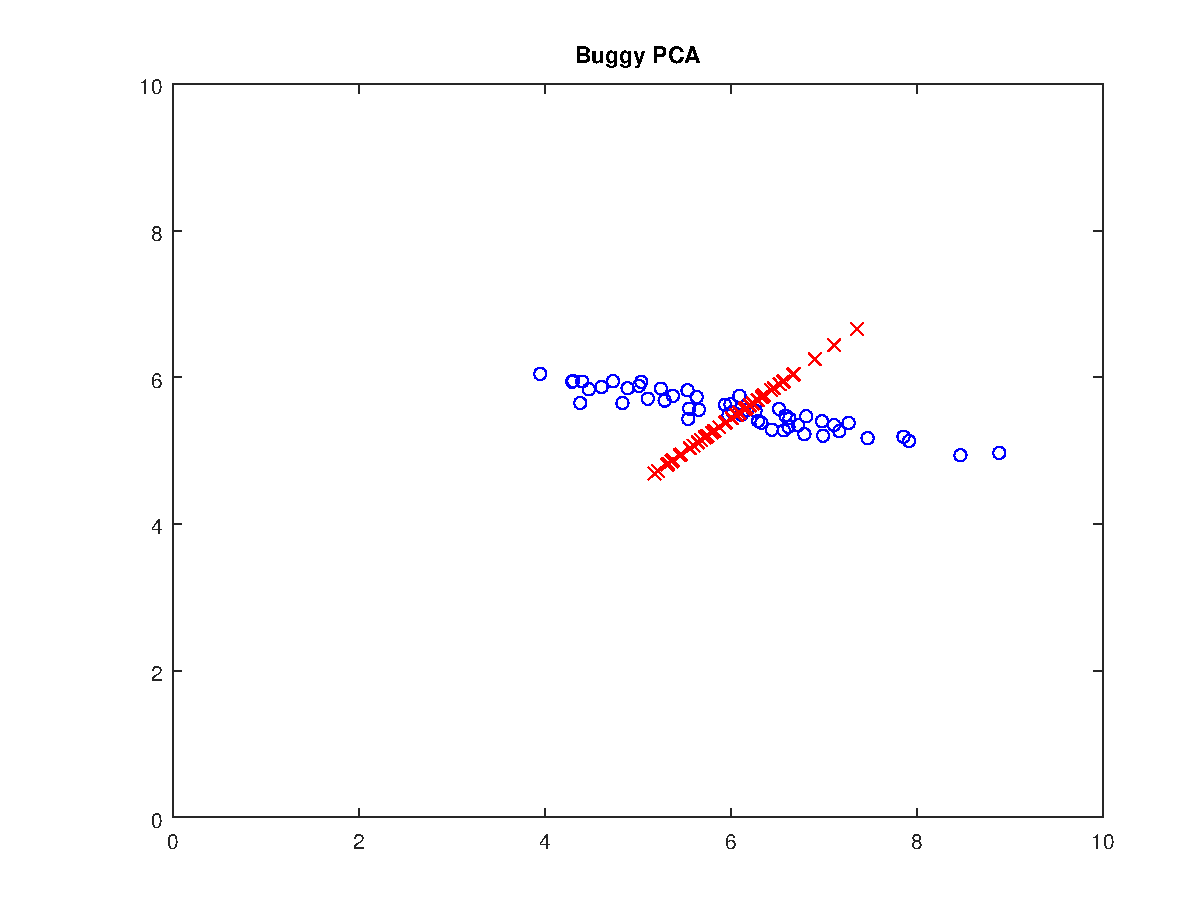
\includegraphics[width=3in]{pcaprog/buggy_pca} \hspace{0.4in}
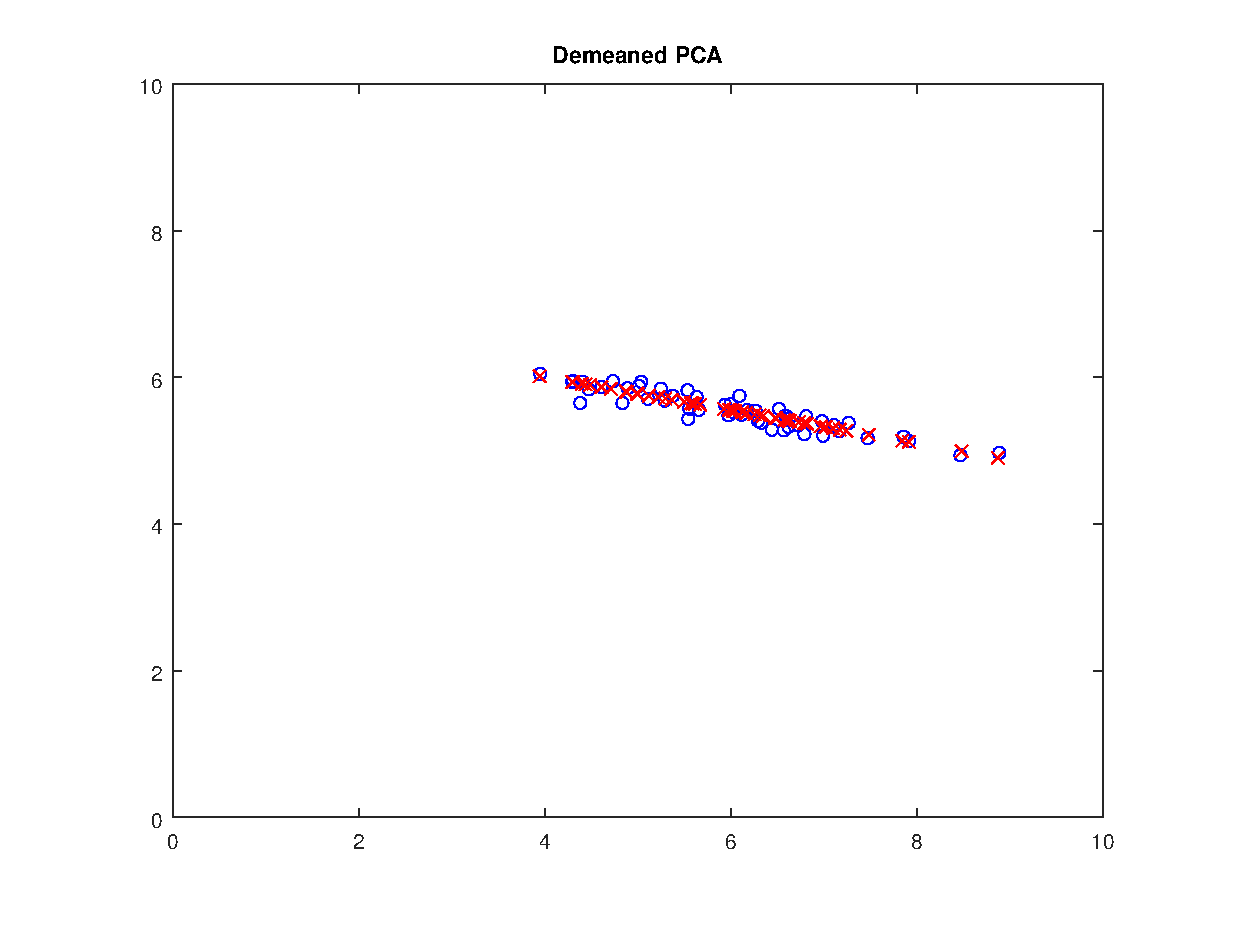
\includegraphics[width=3in]{pcaprog/demeaned_pca} \\
The blue circles are from the original dataset and the red crosses are the reconstructed points.

\begin{soln}
  % insert Fig.png here, title is "knee point"
  \begin{figure}[h]
    \centering
    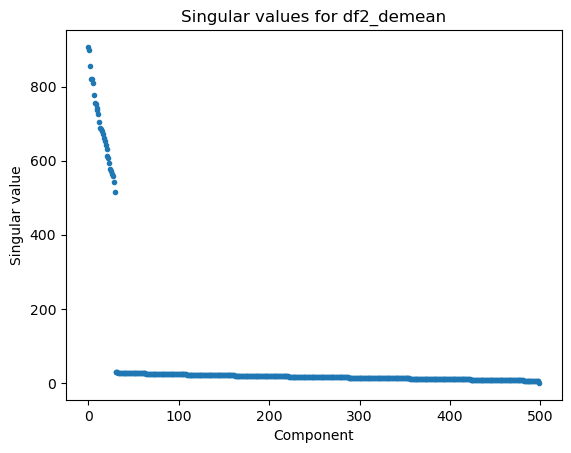
\includegraphics[width=0.5\textwidth]{Fig3.png}
    \caption{Knee point in the singular values of data1000D}
    \label{fig:obj}
  \end{figure}
  From Fig3.png we can see the knee point is 30, so we choose $d=30$.
  In DRLV I set $A_0 = A$ from DRO, and set $\eta_0^2 = \frac{1}{D} tr(cov(X) - AA^\top)$.
  \begin{verbatim}
    Reconstruction Report for data1000D.csv:
    Buggy PCA: 802.7313986203584
    Demeaned PCA: 273.0459589786028
    Normalized PCA: 273.62858099762326
    DRO: 273.0459589786028
    DRLV: 313.69333446428493
  \end{verbatim}
    Q1: Buggy PCA is trying to project the points onto a line that passes through the origin. However, the original points are not seem to on a line passes through the origin, so the reconstruction error is high.
    Q2: No, because these two methods are equivalent to each other. The process of them are both demean, then do SVD, and then project the points onto the first $d$ principal components, finally add the mean back. So the reconstruction error is the same. Their cluster results $z$ are only different in the scale, but the reconstruction results $r(z)$ are the same.
\end{soln}


\vspace{0.2in}



